\section{Simulation Studies and Performance Comparison}
\label{sec:com}

This section discusses the current issues for the existing reconstruction methods and compares the performance between different methods.

\subsection{Geometrical Reconstruction}

The geometrical reconstruction was moved from the plugin to a JANA factory within the GlueX software. 

\subsection{Time-Based Imaging}

An essential part of the time-based imaging is the expected timing spectra for individual pixels (PDFs for individual pixels). As it was discussed in Section~\ref{sec:ti}, these spectra depend on particle direction and velocity, and can be either calculated analytically or simulated.

%Analytical calculation of the expected timing spectra for each pixel relies on the angular resolution for the charged track. (add later)

%Simulation of the expected timing spectra for each pixel requires reasonable grid over the phase space. The photon yield depends on the angles of the charged particle with respect to the radiator sides, and the particle momentum. But we will use the (x,y) position on the DIRC wall and momentum coordinates for the phase space.

To find out the range of the track directions and positions, which can be reconstructed using the same PDF, two simulation studies were performed. A sample of single kaons and pions with momentum of 4 GeV/$c$ and direction defined by the polar angle of $1.4^{\circ}$ and azimuthal angle of $90^{\circ}$ was generated right in front of the DIRC radiator (x = 0, y = -10.4 cm, z = 585.5 cm) and reconstructed using a set of various PFDs. Figure~\ref{pic:simPDF}a shows the resulting separation between pions and kaons when the position of the charged tracks used for PDF was varied. The angle of the tracks used for PDF was kept the same as for the reconstructed sample. Figure~\ref{pic:simPDF}b shows the case when the direction of the tracks used for PDF was varied. In this case the position of the track origin stayed the same as for the reconstructed sample.

\begin{figure}[!h]
\centering
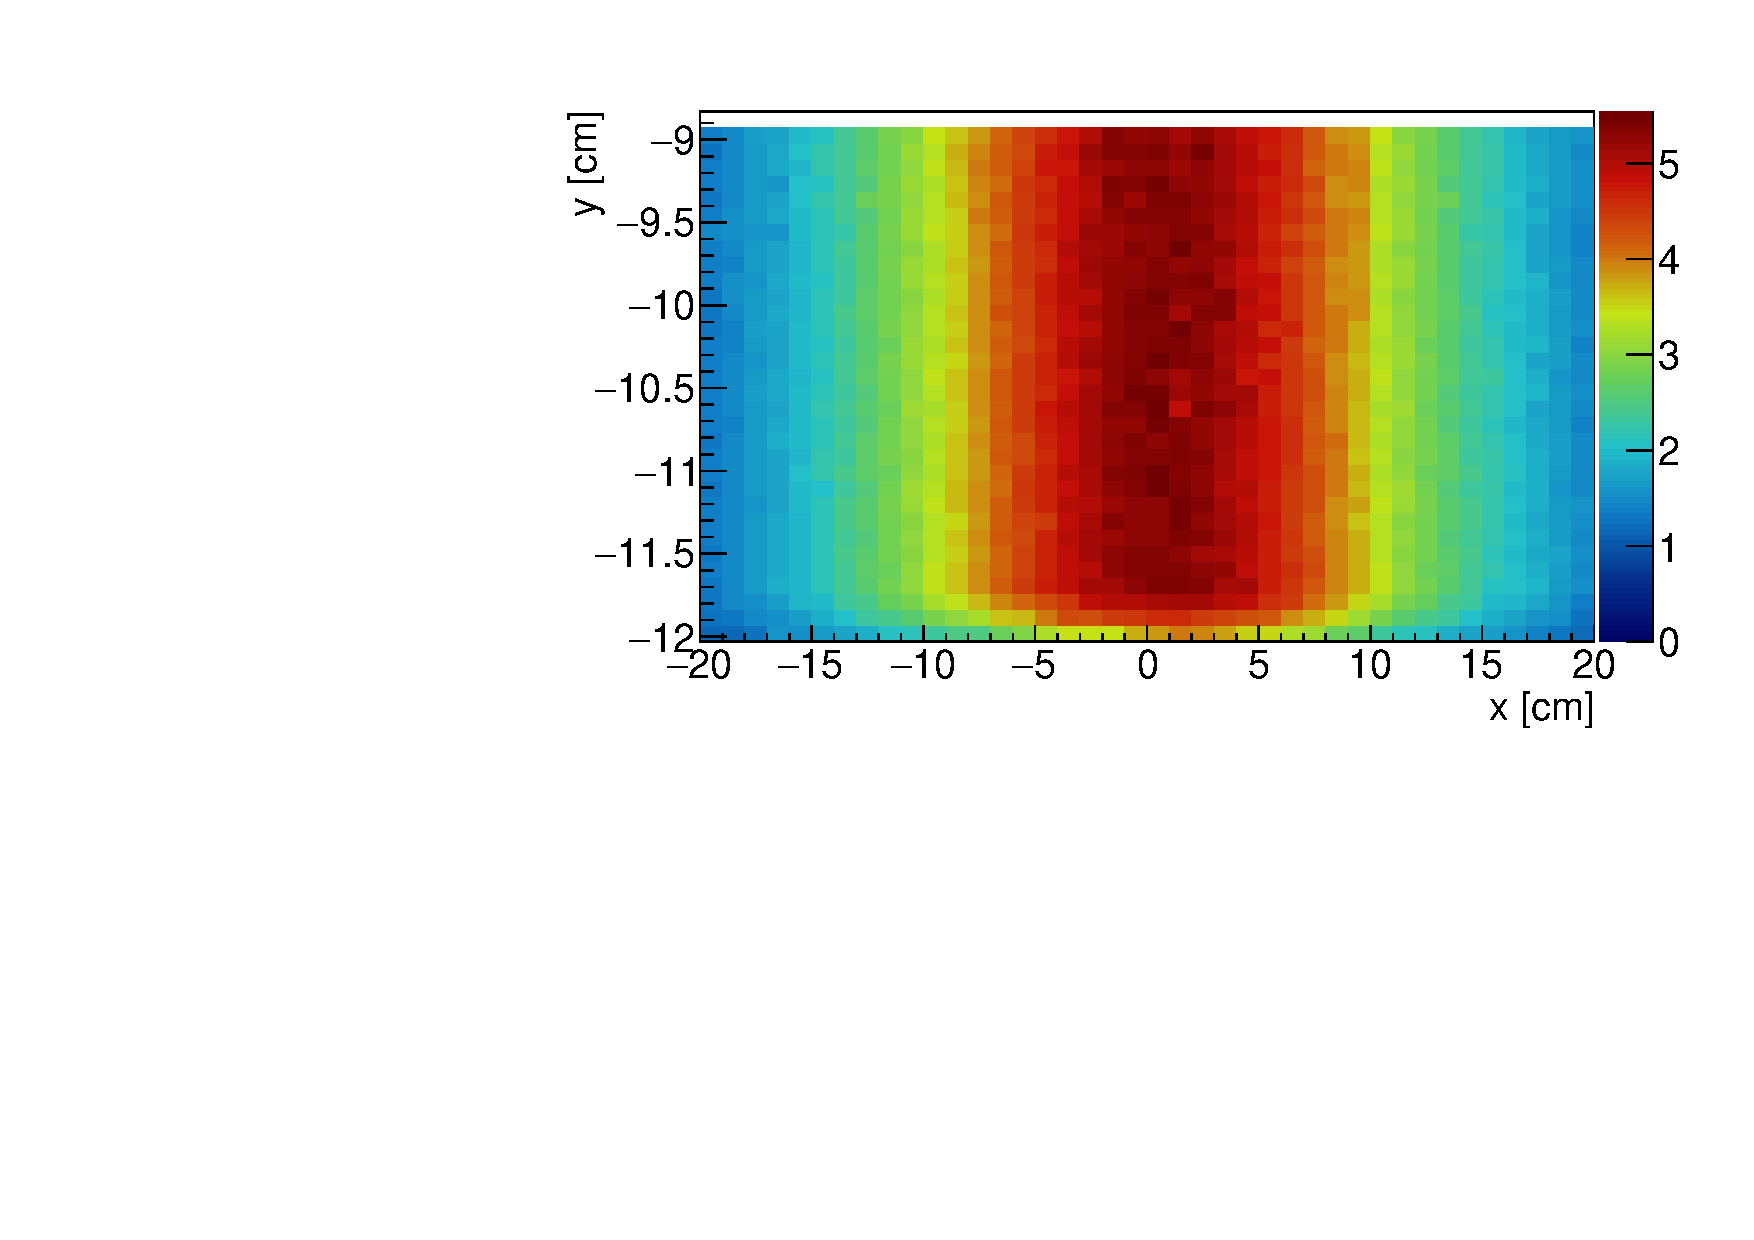
\includegraphics[clip, trim=0.4cm 0.4cm 0.4cm 0.4cm, width=0.45\textwidth]{pics/xy_scan.pdf} \hspace{0.5cm} 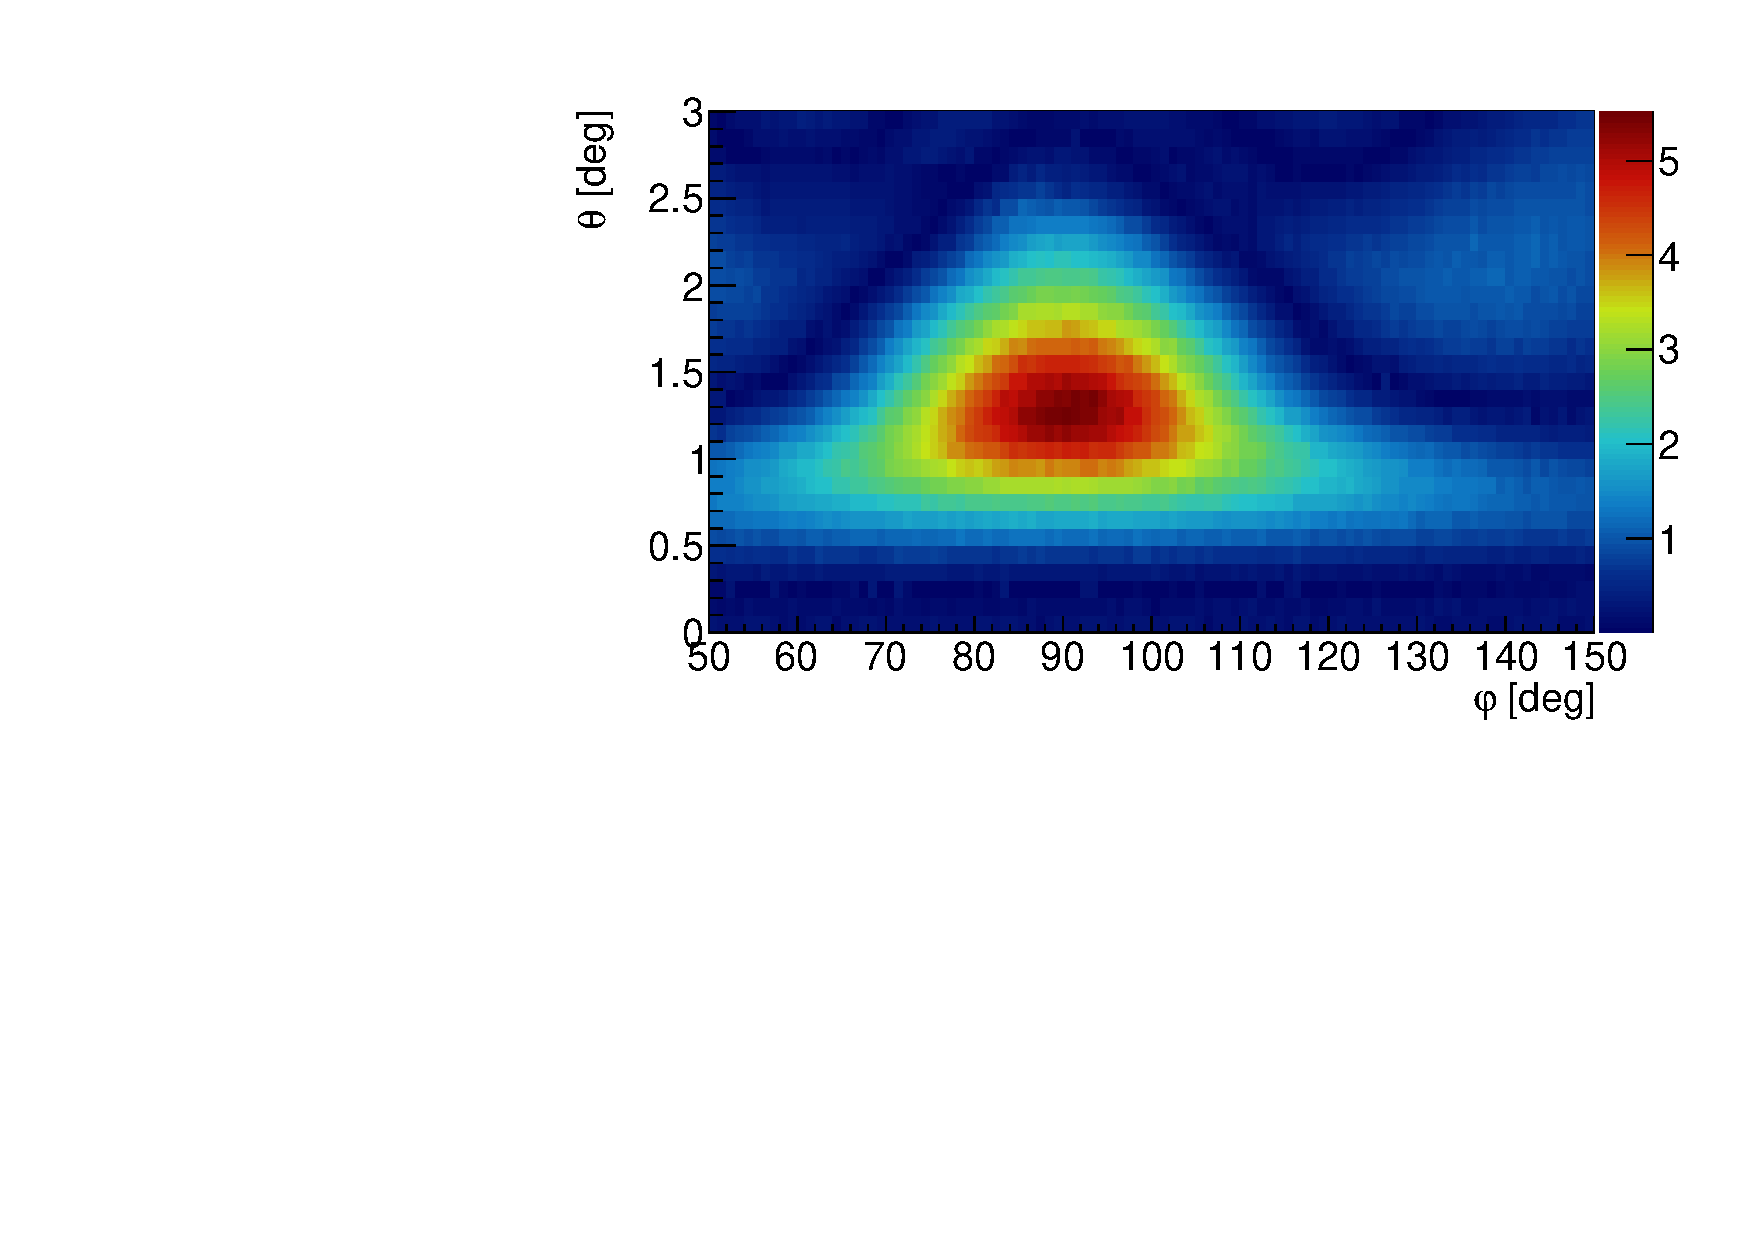
\includegraphics[clip, trim=0.4cm 0.4cm 0.4cm 0.4cm, width=0.45\textwidth]{pics/th_phi_scan.pdf}
\caption{\label{pic:simPDF}
Separation power (color axis) for kaons and pions of a single track event sample (momentum of 4 GeV/$c$, $\theta$ = 1.2$^{\circ}$ and $\phi$ = 90$^{\circ}$ generated right in front of the DIRC radiator with x = 10.4 cm and y = 0) using PDFs for various positions (left) or directions (right). The variation of position for the PDFs kept the direction constant and equal to that for the reconstructed sample. The variation of the angles kept the original position of the tracks constant and equal to that of the reconstructed sample.
}
\end{figure}

The simulation studies show that the separation between pions and kaons does not change if the track is reconstructed using a PDF for the same radiator bar, with x position on the DIRC wall within $\pm$ 5 cm from the track position, and within 0.5 degrees in theta and about $\pm$ 10 degrees in phi.

